
\week{Things That Follow Rules}

Rules are all around us. When you throw a ball into the air, you know
it's going to come down. This is a simple example of a rule.

\hint{You don't need to read the margins, unless you're extra curious!}

% TODO: figure of ball going up and down

Rules can sound boring, but certain rules can be very interesting. In
class, we saw a marble-powered machine made of gates and ramps. Once
the marbles were released, they didn't think -- they just
followed the guides or rules we set up.

This game didn't have any brains, yet its behavior was complex.

This chapter is about simple rules that cause interesting behavior --
without anyone thinking, planning, or deciding.

Even things that seem random run on rules. For example, if you let the
air out of a filled balloon, the balloon will whiz around the
room.
\curious{Even systems that look random often follow perfectly
  strict rules. When a system is sensitive to tiny details, we call it
  \term{chaotic}. This can make prediction hard, even if the rules are
  simple}
Where it lands might seem random, but if you knew the rules
of physics and all the details of how the room was set up, you could
figure out what would happen to the balloon before you let it
go.
\didyouknow{All of known physics can be described by just \emph{nine}
  rules \parencite{motionmountain}!}

You may be wondering what this has to do with computers. The answer
is: \textbf{any system that follows rules is a kind of computer.}

\begin{BigIdeaBox}
A \term{computer} is just a system that follows rules!
\end{BigIdeaBox}

\section{Building a Computer}

When we build a computer, we have to think about the sorts of things
we want to compute.
\huh{Wait! Is everything a computer?}{In nature,
  we discover rules. In computers, we design them. However, some
  scientists really do think of the universe as a kind of
  computer. Others disagree. But it doesn't really matter, because all
  rule-following systems can be studied in the same way. This branch
  of science is called \term{computer science}.}
An extremely simple example of a computer is a lamp. This follows two very simple rules:

\begin{itemize}
\item \textcolor{IdeaBlue}{\textbf{Rule 1}} - When you flip the switch on, the light goes on.
\item \textcolor{IdeaBlue}{\textbf{Rule 2}} - When you flip the switch off, the light goes off.
\end{itemize}

Usually, we only call something a computer if it does more interesting
things. To make computers like that, we have to set up the rules
carefully.  \curious{A lamp follows rules, but it cannot store
  information or combine rules in new ways. What separates simple
  machines from powerful computers is not just the number of rules,
  but how rules combine.}

\subsection{Turing Tumble}

The \emph{Turing Tumble} game lets you set up a system that follows
simple rules. The game has two colors of marbles: blue on the left and
red on the right. The marbles fall down and hit different pieces along
the way.

Each piece follows a simple rule. Some pieces always send marbles the
same direction. Other pieces can change what they do depending on what
happened before. When a marble reaches the bottom, it can hit a lever
that releases a new marble.\didyouknow{It may seem crazy, but this is
  \emph{exactly} how real computers are built. Instead of marbles,
  engineers use even smaller balls called electrons.}

By changing how the pieces are laid out, you can make interesting
computers.

\begin{figure}[ht]
\centering

\begin{tikzpicture}
  \TTBoard[cols=8,rows=10,unit=7mm,pegs=true,label={A board that follows rules}]

  % Place a Bit at (col=3,row=6) with state 0
%  \TTBit[state=0]{3}{6};

  % Marbles
  \TTMarble{1}{10}
  \TTMarble{1}{9}

  % A simple incoming path and the two possible outputs
  \TTArrow{1}{10}{2}{9}
  \TTArrow{2}{9}{3}{8}
  \TTArrow{3}{8}{3}{7}
%
%  % Rule arrows for the Bit: solid=0 path, dashed=1 path
  \TTArrow[style={thick},label={if 0}]{3}{6}{2}{5}
  \TTArrow[style={thick},label={if 1}]{3}{6}{4}{5}
\end{tikzpicture}

\caption{What happens to this machine when a blue marble drops down? Can you identify the rule? See the bottom of the page for the answer.\upfootnote{The switch flips back and forth}}
\end{figure}

There are several different elements that you can place on the Turing
Tumble board.

\termheading{The Bit}

The \emph{bit} piece can point either left or right. If the bit is
pointed to the left, the next marble that hits it goes left and the
bit flips right. If the bit is pointed right, then the next marble
that hits it goes right and the bit flips left.  \curious{A single bit
  stores the answer to one yes/no question. Real computers are built
  from quadrillions of bits working together.}

The bit is special because it changes what happens the \emph{next
time} the program runs.\curious{When a program can change behavior
  based on something that happened before, we say it has
  \term{state}.}

\termheading{The Ramp}

The \emph{ramp} sends marbles either left or right, depending on how its
placed on the board. A ramp facing one way always sends marbles down
that way. Ramps do not flip after a marble passes by. \curious{When a
  behavior does not change, we call it \term{pure}.}

\termheading{The Crossover}

The \emph{crossover} prevents marbles from hitting each other. When
two marbles hit a crossover at the same time, instead of colliding,
the crossover redirects them so they pass safely through.

\termheading{The Interceptor}

The \emph{interceptor} is a piece that can be open or closed. If
closed, the marble stops. If open, the marble passes through. This
piece lets you turn machines on or off based on what happened earlier.

\termheading{Gears}

Some pieces, like interceptors, can be in multiple positions. Gears
let us move these pieces. The \emph{gear bit} acts like a bit, but
also moves a gear that can move other pieces, such interceptors. This
lets one part of the machine \emph{change the behavior} of another
part.\curious{When one part of a system changes another part, we call
  this \term{feedback}. Feedback is how machines can control
  themselves.}

\begin{BigIdeaBox}
  Each piece follows a very simple rule, but combining them together,
  we can build many different kinds of computers.
\end{BigIdeaBox}

\section{From Marbles to Code}

It may not seem like it, but Turing Tumble is a \emph{real
computer}. It's not the only day to build one though, and most
computers today use electricity.
\begin{marginfigure}
  \includegraphics[width=0.8\linewidth]{../Week1/figures/alan-turing.jpg}
  \caption{\textbf{Alan Turing} (1912-1954) asked ``What can machines do if they follow
    rules''?. The name \emph{Turing Tumble} comes from Alan Turing. }
\end{marginfigure}

Inside a modern computer, tiny moving things called \emph{electrons}
flow through parts that follow simple rules, just like the pieces on
the Turing Tumble board. Some parts remember things, some parts make
decisions, and some parts make sure electrons move in the right
direction.

\begin{BigIdeaBox}
  Whether it uses marbles or electricity, a computer is just a system
  that follows rules.
\end{BigIdeaBox}

Modern computers are so complicated that you don't need to physically
move pieces to make them do new things. Instead, computers are built
so that they can follow many different rules depending on what you ask
them to do.\curious{Every computer has a basic set of rules that
  depends on the physical parts inside it. Programming languages like
  Python are built on top of these rules, but we don't need to worry
  about them yet. This hidden layer of rules is sometimes called the
  \term{computer architecture}.}

The process of telling a computer which rules to follow is called
\term{programming}. There are many ways to program a computer. In the
Turing Tumble game, we moved pieces physically. On modern computers,
we use a special language called a \term{programming language}.

One of the simplest programming languages to start with is called
\term{Python}.\aside{Don't worry, it's not this kind of Python!}

\subsection{Talking to a Computer}

In this class, we will use the \textbf{Thonny} Python environment.
\aside{Thonny can be downloaded at \href{https://thonny.org}{https://thonny.org}.}

\begin{figure}
  \label{fig:thonny-interface}
  \centering
  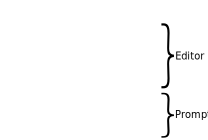
\includegraphics[width=0.9\linewidth]{../Week1/figures/thonny-interface.pdf}
  \caption{The Thonny interface. The interface is split into two
    parts: (1) the editor and (2) the prompt.}
\end{figure}

We can talk to Python by entering ``rules'' into the prompt (see
\prettyref{fig:thonny-interface}) and immediately seeing what
happens. This is like dropping a marble into the machines we built
earlier and watching what happens.  \didyouknow{Long before modern
  computers, scholars attempted to study \emph{human} language through
  using rules. One such scholar was the Indian grammarian
  P\={a}\d{n}ini. Around 500 BC, he described the Sanskrit language
  using a precise set of rules that could combine to generate all
  valid sentences in that language!}

In Turing Tumble, our rules were made of plastic pieces. In Python, we
use special words and symbols to write rules.

Let's type our first rule! The simplest rules (also known as \term{expressions})
are the ones that stand for numbers. We can enter these rules by
typing in a number and pressing the Enter or Return key.

Try entering these into the Thonny prompt, and see what
happens.\hint{Type each line one at a time and observe what happens.}

\begin{replbox}
1<ENTER>
54<ENTER>
0<ENTER>
\end{replbox}
\hint{The response from the computer to each of these should be
  numbers. If it's not, you may have typed it in incorrectl. Try it
  again. If that still doesn't work, see \prettyref{sec:errors}}

The rule for numbers is that when you enter them in, you get the same
number out!

\begin{BigIdeaBox}
  Just like the balloon thrown up in the air, and just like the
  machines we built, every time you run these rules, the answer is the
  same.
\end{BigIdeaBox}

Let's try something more complicated. Before trying the following
rules, think about what is going to happen. A good programmer tries to
predict the output before they use the rule.  \curious{When you type
  something into Python and press Enter, the computer always produces
  the same result for the same input. This idea is called
  \term{determinism}.}

\begin{replbox}
1 + 1<ENTER>
5 - 3<ENTER>
4 * 3<ENTER>
\end{replbox}

\subsection{How Computers Follow Rules}

The symbols we used above connected two number rules together. When we
pressed enter, we got a new number, which is itself a kind of
rule. The way this number was generated depended on the exact symbol
we used. You're probably familiar with the \code{+} symbol, which
means addition. Can you guess what the \code{*} symbol stands for?
If you guessed multiplication, you're right. \hint{You're probably
  familiar with the symbol $\times$ for multiplication, but that
  symbol is hard to type! Most programming languages use \code{*} to
  denote multiplication.}

Since Python lets us combine rules however we want, we can combine
rules involving both multiplication and addition. Before trying the
exercises below, try to guess what the answer is and write down why.

\begin{replbox}
4 + 2 * 3<ENTER>
2 * 3 + 4<ENTER>
\end{replbox}

You may be surprised that the these rules both produced the same number.

In many programming languages, including Python, symbols like
\code{+} and \code{*} have rules to determine which one goes
first. In this case, multiplication always goes first.\curious{\term{Operator precedence} rules determine which written rules get done first.}

Sometimes it can help to \emph{draw} the expressions to figure out
exactly what is going on.

% TODO figure that shows how to make these into trees

What if we want to make additions occur first? We can always use
parentheses (that is \code{(} and \code{)}) around rules we want to
execute first.

\begin{replbox}
2 * 3 + 4<ENTER>
2 * (3 + 4)<ENTER>
\end{replbox}\hint{Remember it's always a good idea to \emph{predict} what is going to happen \emph{before} hitting the Enter key.}

In this case, the parentheses force the \code{3 + 4} rule to execute
first. \prettyref{fig:parenrules} shows how the diagram for this rule
looks different than the diagram for the \code{2 * 3 + 4} rule.

\begin{figure}
  \label{fig:parenrules}
  % TODO add figure
  \caption{The rule \code{2 * (3 + 4)} is drawn differently than the rule \code{2 * 3 + 4}.}
\end{figure}

\begin{BigIdeaBox}
  When rules combine, there are rules to determine which rule go
  first. No matter which rules we are talking about, they always
  behave in \emph{exactly} the same way.
\end{BigIdeaBox}

There's one more thing to think about. What if we put parentheses
around the multiplication?

\begin{replbox}
2 * 3 + 4<ENTER>
(2 * 3) + 4<ENTER>
\end{replbox}
\hint{At this point, you probably know you need to \emph{predict} what is going to happen before proceeding!}

In this case, it again helps to draw it out. As you can see both of
these rules can be represented by the same diagram (see
\prettyref{fig:paren-mult}). Since the diagrams match, the rules mean
the same thing even though they're typed out differently.
\curious{Electronic computers are structured as layers of rules. A
  really hard-working computer programmer made rules that told Python
  what to do to understand the rules you type in to the
  computer. Those rules were typed out in another language called
  C. Another program called a \term{compiler} took those rules and
  generated yet more sets of rules. Its rules all the way down!}

\begin{BigIdeaBox}
  The same rule can be typed out many different ways! We can apply the
  rules for diagramming rules to see if they mean the same
  thing.
\end{BigIdeaBox}

\begin{figure}
  \label{fig:paren-mult}
  % TODO add figure
  \caption{The rule \code{2 * 3 + 4} and \code{(2 * 3) + 4} are
    represented by the same diagram even though they are typed out
    differently.}
\end{figure}

\subsection{Rules with Words}

So far, all our rules have involved numbers, but computers can handle
more than that. Computers can also follow rules about
\emph{words}.\didyouknow{Python actually has \emph{two} kinds of
  numbers, but we will have to come back to that later.}

\begin{replbox}
"hello"<ENTER>
"my name is Bob"<ENTER>
\end{replbox}
\hint{Words must be surrounded by \code{"}s or you will get an
  error. Make sure you type everything in exactly as written.}

You'll notice that Python responds back with the word (or phrase) you
put in. \didyouknow{Programmers use the term \term{strings} to refer to
  rules representing words in programs.}

Now try this, but remember to \emph{predict} what is going to happen
before typing it in.

\begin{replbox}
"hello " + "world"<ENTER>
\end{replbox}

Did it do what you expected? If you typed it in correctly, Python
should have responded with \code{"hello world"}.\huh{But I thought
  \code{+} added numbers together. How come I can use it with
  words?}{Some symbols like \code{+} can do different things depending
  on whether it is used with words or numbers. Different programming
  languages have different rules regarding which combinations of
  simbols, words, and numbers are allowed and what exactly they
  mean. The technical term for this is \term{operator overloading}. A
  useful list of these rules in Python is given in
  \prettyref{tab:operator-rules-1}}

We've now seen a rule involving words! When you use \code{+} on two
words, you get those two words put together. What else can we do with words?

\begin{replbox}
"ho" * 3<ENTER>
\end{replbox}

You should see the response \code{"hohoho"}, which is just \code{"ho"}
repeated three times. \hint{Python did not suddenly decide to be
  festive. The word returned is the result of Python applying its set
  of rules \emph{exactly} to what you wrote.}

\begin{TryThisBox}
Can you multiply a word by another word? What would this mean? Think
about it, before we find out the answer in the next section.
\end{TryThisBox}

\subsection{Some Rules Don't Make Sense}

Remember that when we type rules, Python applies more rules to make
sense of what we typed. We can visualize these rules by drawing
diagrams. But sometimes, we write something that Python's rules cannot
figure out. Although we can type them using the keyboard they don't
make sense to Python. This would be like trying to place two Turing
Tumble pieces on one peg when building a machine -- it just doesn't
make sense. We call these issues \term{syntax errors}.

\begin{replbox}
2 + 5 +<ENTER>
* 4<ENTER>
\end{replbox}

Other times we type rules that Python understand, but when it tries to
process them, it gets confused. This is like placing a much larger
marble into the Turing Tumble game -- although our placement of pieces
makes sense, we cannot make the pieces move with the wrong type of
marble. This is called a \term{runtime error}. You may have also heard
it called a \term{bug}. \didyouknow{The first computer bugs were
  caused by actual bugs that got stuck in hot electronic parts used in
  the earliest electric computers. Yuck!}

Both of these issues are kinds of \term{errors}.

In Python, errors are reported back to us as they occur, and Python
tries to give us information that can help us correct the error.
\hint{Although it may seem scary, there is nothing ``wrong'' with an
  error. It's just the computer applying rules and telling you
  something doesn't make sense.}

Although Python will provide some information that can be useful to
fix our program, Python is itself a collection of rules, and its rules
may not fully understand what we are trying to do based on what we
input. This is where the job a programmer becomes important.

\begin{BigIdeaBox}
  Python always applies the same rules to understand and process our
  rules, but sometimes what we put in doesn't make sense.
\end{BigIdeaBox}

\section{Conclusion}

Computers follow rules exactly. When we program a computer, we make
new rules for the computer to follow. In Python, simple rules can
involve numbers and words. Sometimes, the rules we write don't make
sense. This is called an error, but is still the result of the
computer following a set of rules.

We haven't learned how to program \emph{yet}, but we have started
toying with the idea of turning ideas into instructions. When we do
this, the small details really matter. Missing pieces can cause
confusion. Unclear instructions lead to unexpected results. When
things go wrong, it's not because the computer was wrong, but because
it followed the instructions exactly as written.

This is computer's greatest strength. They never guess or fill in
missing steps. They just do exactly what you tell it! Computer science
is not about memorizing commands or tying a lot. It's about learning
how to say things clearly enough that a process -- whether a table
game, machine, or a person -- can follow your ideas without confusion.

In the next chapter we'll start to think deeper about how to precisely
describe to the computer the things we want to make.

\Exercises

\curious{Exercises are fun things you can try at home}

\begin{exercises}
\item Construct Turing Tumble boards that do the following:
  \begin{enumerate}
  \item Send the marble down the opposite end
  \end{enumerate}

\item Figure out the rule that the following Turing Tumble boards follow:
  \begin{enumerate}
  \item Test
  \end{enumerate}

\item Predict the answer to the following Python rules:
  \begin{enumerate}
  \item \code{1 \enterkey}
  \item \code{-1 \enterkey}
  \item \code{3 + 2 \enterkey}
  \item \code{3 * 9 + 6 \enterkey}
  \item \code{6 * 3 * 2 \enterkey}
  \item \code{6 + 3 + 2 \enterkey}
  \item \code{6 * 4 - 8 * 2 \enterkey}
  \item \code{6 * 4 // 2 \enterkey}\hint{Remember that \code{//} means division in Python}
  \end{enumerate}
  \answer{1,-1,5}

\item Try the following rules.
  \begin{enumerate}
  \item \code{len(``a'')}
  \item \code{len(``ab'')}
  \item \code{len(``abc'')}
  \item \code{len("")}
  \end{enumerate}
  What does the \code{len} rule do?
\end{exercises}

\begin{largetable}
  \caption{This is a list of symbols you can use to combine rules in
    Python. Symbols that appear first are executed first, unless you
    use parentheses to force some rules to ge first. The behavior of
    symbols can depend on whether it's used with numbers or words. All
    these variants are given here}
  \label{tab:operator-rules-1}
  \begin{tabularx}{\linewidth}{llL}
      \toprule
      \headercol{Symbol} & & \headercol{Meaning} \\\midrule
      {\ttfamily *, //, \%} & \code{number * number} & Multiply two numbers together \\
      & \code{number // number} & Divide two numbers \\
      & \code{number \% number} & The remainder when dividing the numbers \\
      & \code{word * number} & Repeat the word this many times \\\hline
      {\ttfamily +, -} & \code{number + number} & Add two numbers together \\
      & \code{number - number} & Subtract the second number from the first \\
      & \code{word + word} & Combine the two words together \\\bottomrule
  \end{tabularx}
\end{largetable}
